\documentclass[12pt, answers]{exam}
\usepackage{tikz}
\usepackage{amsmath}
\usepackage{amsfonts}
\usepackage{amssymb}
\usepackage{graphicx}
\usepackage{multirow}
\usepackage{enumitem}
\usepackage{subfiles}
\usepackage[most]{tcolorbox} 
\usepackage{changepage} % for adjustwidth
\usepackage{xepersian}

\settextfont[
    Path = ../fonts/,
    Scale = 1.0,
    BoldFont = *Bd,
    ItalicFont = *It,
    BoldItalicFont = *BdIt,
    Extension = .ttf
]{XB Yas}

\renewenvironment{solution}{%
  \par
  \begin{tcolorbox}[
    breakable,                
    colback=white,
    colframe=black,
    arc=1pt,
    boxrule=0.6pt,
    left=4mm, right=4mm,
    top=2mm, bottom=2mm,
    before skip=10pt,
    after skip=10pt,
    segmentation style={solid, black}, 
    before upper={\noindent\textbf{\color{blue}پاسخ:}\par\vspace{0.5em}}
  ]
 }
{%
  \end{tcolorbox}
  \vspace{1em}
}

% Wide solution environment (extends into the question label area)
% Usage: replace \begin{solution} ... \end{solution} with \begin{widesolution} ... \end{widesolution}
% Keeps the same optional title argument as exam's solution: \begin{widesolution}[عنوان]
\newenvironment{widesolution}[1][]{%
    \begin{solution}[#1]%
    % Outdent left by the current list left margin so the solution spans full text width
    \begin{adjustwidth}{\dimexpr-\leftmargin\relax}{0pt}%
}{%
    \end{adjustwidth}%
    \end{solution}%
}

\renewcommand{\solutiontitle}{\noindent\textbf{\color{blue}پاسخ:}\par}
\newcommand{\class}{اصول سیستم‌های عامل}
\newcommand{\term}{نیم‌سال اول ۰۴-۰۵}
\newcommand{\college}{دانشکده ریاضی و آمار}
\newcommand{\prof}{استاد: دکتر رفیعی}
\newcommand{\group}{نام دانشجو}

\begin{document}
%%%%%%%%%%%%%% HDR START 
\pagestyle{head}
\firstpageheader{}{}{}
\runningheader{صفحه \thepage\ از \numpages}{}{\class}
\runningheadrule
\begin{tabular}{p{.7\textwidth} l}
    \multicolumn{2}{c}{\textbf{به نام خدا}}                                            \\
                    & \multirow{2}{*}{
\includegraphics[scale=0.2]{../UILOGO.png}} \\
    \textbf{\class} &                                                                  \\
    \textbf{\term}  &                                                                  \\
    \textbf{\prof}  &                                                                  \\
    \textbf{\group} &                                                                  \\
                    & \textbf{\college}
    \\
    % & \textbf{\todaydate} \\
    % & \textbf{\deadline} \\ \\
\end{tabular}\\
\rule[1ex]{\textwidth}{.1pt}

\begin{center}
    \textbf{\lr{Problem Set 1}}
\end{center}
%%%%%%%%%%%%%% HDR END 


\begin{questions}
    \pointpoints{نمره}{نمره}

    %%%%%%%%%%%%%% 1 START 
    \question به سوالات زیر پاسخ کامل دهید:
\begin{parts}
    \part[5]  تفاوت سیستم‌های خوشه‌ای و سیستم‌های چند پردازنده‌ای چیست؟ دو ماشین متعلق به یک خوشه چه همکاری‌ای باید داشته باشند تا سرویس خوبی فراهم شود؟
    \part[5]  هدف وقفه چیست؟ تفاوت‌های بین وقفه و تله چیست؟ آیا تله می‌تواند به دلخواه توسط برنامه‌نویس تولید شود؟ اگر بلی، برای چه هدفی؟
    \part[5]  معماری NUMA چیست و چرا زمان دسترسی پردازنده‌ها به حافظه در این معماری یکسان نیست؟
    \part[10]  در چه حالتی استفاده از چندبرنامگی به جای چند وظیفگی راندمان سیستم کامپیوتری را افزایش می‌دهد؟
    چنین سیستمی برای چه کارهایی مناسب‌تر است؟
\end{parts}


    \begin{solution}
        \begin{parts}
            \part    سیستم‌های چندپردازنده‌ای یک کامپیوتر با چند پردازنده هستند که حافظه و منابعش را به‌صورت مشترک استفاده می‌کنند و ارتباط بین پردازنده‌ها از طریق حافظه یا باس سیستم است. این سیستم‌ها مقیاس‌پذیری محدودی دارند و خرابی یک پردازنده می‌تواند کل سیستم را تحت تأثیر قرار دهد.
            در مقابل، سیستم‌های خوشه‌ای از چند کامپیوتر مستقل تشکیل شده‌اند که از طریق شبکه به هم متصل‌اند و هر گره حافظه و منابع خودش را دارد. این سیستم‌ها مقیاس‌پذیرتر و مقاوم‌تر در برابر خطا هستند، زیرا اگر یک گره خراب شود، بقیه گره‌ها می‌توانند سرویس را ادامه دهند.
            برای ارائه سرویس با دسترس‌پذیری بالا، دو ماشین در یک خوشه باید سلامت یکدیگر را پایش کنند، مکانیزم failover داشته باشند تا در صورت خرابی یکی، دیگری سرویس را ادامه دهد، داده‌ها را همگام نگه دارند و ارتباط مطمئن بین گره‌ها برقرار باشد. همچنین باید از تجهیزات و شبکه افزونه استفاده شود و سرویس نرم‌افزاری قابلیت خوشه‌بندی و failover را داشته باشد.

            \part وقفه‌ها (Interrupts) سیگنال‌هایی هستند که به پردازنده می‌گویند اجرای کار جاری را متوقف کرده و یک رویداد فوری را پردازش کند. این کار باعث می‌شود سیستم بتواند به سرعت به دستگاه‌ها یا خطاهای سخت‌افزاری پاسخ دهد و CPU هم بیهوده منتظر نماند.
            تله‌ها (Traps) تفاوت مهمی با وقفه دارند؛ تله‌ها همزمان با اجرای یک دستورالعمل رخ می‌دهند و معمولاً به دلیل یک خطا یا درخواست برنامه برای استفاده از خدمات سیستم عامل ایجاد می‌شوند.
            بله، برنامه‌های کاربر می‌توانند عمداً تله ایجاد کنند تا با سیستم عامل تعامل کنند، مثلاً برای خواندن یا نوشتن فایل یا ایجاد فرایند جدید.

            \part NUMA مخفف
            \lr{Non-Uniform Memory Access}
            است.
            در این معماری هر پردازنده به یک بخش محلی از حافظه نزدیک‌تر است و دسترسی به آن سریع‌تر انجام می‌شود. اما اگر پردازنده بخواهد به حافظه‌ی بخش دیگری (
            \lr{Remote Memory}
            ) دسترسی پیدا کند، زمان بیشتری لازم است. به همین دلیل زمان دسترسی حافظه برای همه پردازنده‌ها یکسان نیست.

            \part چندبرنامگی زمانی از چندوظیفگی کارآمدتر است که هدف اصلی بیشینه‌سازی توان (throughput) پردازنده باشد و نیاز به پاسخ‌گویی تعاملی کاربران وجود نداشته باشد. دلیلش این است که چندوظیفگی برای ایجاد تعامل، از سوئیچ‌های زمانیِ مکرر استفاده می‌کند که هر سوئیچ
            (\lr{context-switch})
            هزینهٔ
            و سربار دارد؛ در حالی که در حالت چندبرنامگی سوئیچ‌ها عموماً زمان‌مند نیستند (ایجاد می‌شوند وقتی یک فرایند مسدود شود) و در نتیجه سربار کمتری برای پردازنده ایجاد می‌شود.

            چنین سیستمی برای کارهای زیر مناسب است:
            \begin{itemize}
                \item پردازش دسته‌ای \lr{(batch processing)} داده‌های حجیم
                \item محاسبات عددی/شبیه‌سازی‌های علمی که هدفشان کارکرد طولانی و بدون دخالت کاربر است.
                \item رندرینگ و تبدیل رسانه \lr{(render, encode)} که باید بیشترین استفادهٔ CPU را داشته باشند.
                \item صف‌های کاری \lr{(job queues)} و سرویس‌های پردازش حجم بالا که اولویت روی throughput است.
            \end{itemize}
        \end{parts}
    \end{solution}
    %%%%%%%%%%%%%% 1 END 

    \pagebreak

    %%%%%%%%%%%%%% 2 START
    \question[20]  تصور کنید شما طراح یک سیستم‌عامل جدید هستید و به دلایل عملکردی تصمیم گرفته‌اید اجرای دو حالته
    (\lr{User Mode} و \lr{Kernel Mode})
    را حذف کنید. در این سیستم همه برنامه‌ها مستقیماً به سخت‌افزار و حافظه کامل دسترسی دارند.
    \begin{enumerate}
        \item تحلیل کنید چه مشکلات امنیتی، پایداری و همزمانی ممکن است ایجاد شود.
        \item توضیح دهید یک برنامه مخرب چگونه می‌تواند از این ضعف برای دسترسی به حافظه برنامه‌های دیگر، خراب کردن فایل‌ها یا مختل کردن سیستم سوءاستفاده کند.
        \item اگر بخواهید بدون برگرداندن حالت کرنل، سطحی از امنیت و کنترل منابع را حفظ کنید، چه روش‌های جایگزینی پیشنهاد می‌کنید؟
        \item توضیح دهید اجرای دو حالته چگونه این مشکلات را به شکل ساده‌تر و مؤثرتری حل می‌کند.
    \end{enumerate}

    \begin{solution}
        \begin{parts}
            \part حذف اجرای دو حالته باعث ایجاد مشکلات جدی امنیتی و پایداری می‌شود. برنامه‌های مخرب می‌توانند به حافظه سایر برنامه‌ها دسترسی پیدا کنند، داده‌ها را تغییر دهند یا سیستم فایل را خراب کنند. مدیریت همزمانی و اشتراک منابع سخت‌تر شده و احتمال کرش سیستم افزایش می‌یابد.
            \part برنامه مخرب می‌تواند مستقیماً به آدرس‌های حافظه سایر برنامه‌ها دسترسی پیدا کند، داده‌ها یا کد آن‌ها را تغییر دهد، فایل‌ها را پاک یا خراب کند و عملکرد سیستم را مختل کند.
            \part می‌توان از Virtualization، Sandbox، حفاظت حافظه
            \lr{(Memory Protection)}
            یا کنترل سخت‌افزاری دسترسی به منابع استفاده کرد تا برنامه‌ها از هم ایزوله شده و سطح کنترل حفظ شود.
            \part اجرای دو حالته باعث می‌شود برنامه‌های کاربر در حالت محدود اجرا شوند و سیستم‌عامل کنترل کامل روی دسترسی به منابع و حافظه داشته باشد. این روش امنیت و پایداری را تضمین کرده و مدیریت همزمانی و اشتراک منابع را ساده‌تر می‌کند.
        \end{parts}

    \end{solution}
    %%%%%%%%%%%%%% 2 END

    \pagebreak

    %%%%%%%%%%%%%% 3 START
    
\question آقا
طرفای صفحه ۸ اسلاید ۴ یه دیاگرامی بود که خیلی شیک اسکیپ کردید. چی میگفت
حالا؟ داشت نشون می‌داد که اگر وسط کار
CPU
عزیز یه وقفه ایجاد بشه، روند انجام کارها به چه صورت پیش می‌رِد!
چون حوصله باز کردن اسلاید‌ها رو ندارید عکسشو میذاریم اینجا:
\begin{center}
    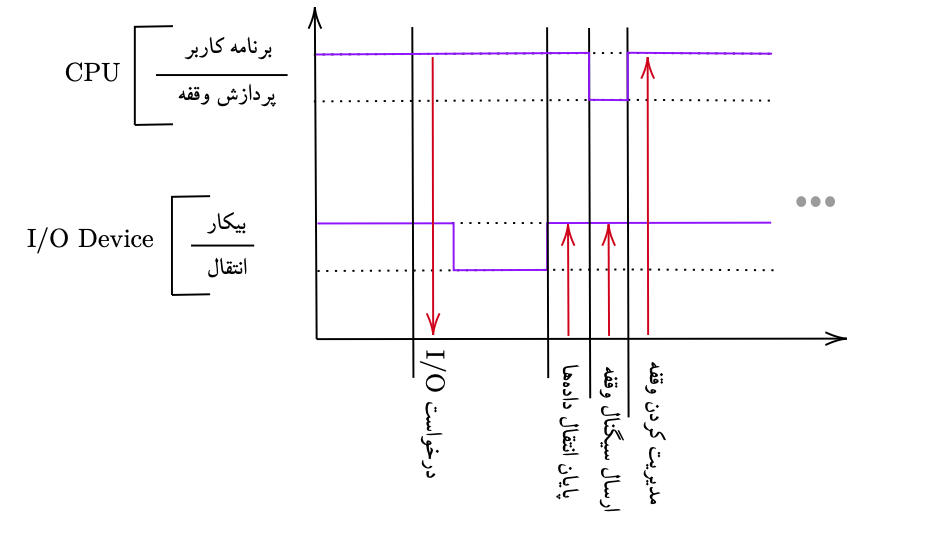
\includegraphics[scale=0.9]{images/diagram.png}
\end{center}

اول خوب تحلیلش کنید و بعد سناریوی زیر رو بخونید:
\begin{enumerate}
    \item یک فرایند کاربر که روی CPU در حال اجراست، یک درخواست ورودی/خروجی (I/O) به دیسک ارسال می‌کند. به جای اینکه CPU هر انتقال داده را با وقفه‌ها مدیریت کند، از
          \lr{DMA (Direct Memory Access)}
          استفاده می‌کند.
    \item وقتی درخواست I/O داده می‌شود، CPU کنترلر DMA را برنامه‌ریزی کرده و سپس اجرای فرایند کاربر را ادامه می‌دهد.
    \item کنترلر DMA انتقال داده‌ها بین حافظه و دستگاه ورودی/خروجی را مستقیماً برعهده می‌گیرد، در حالی که CPU آزاد است تا دستورهای کاربر را اجرا کند.
    \item وقتی انتقال کامل شد، کنترلر DMA یک وقفه به CPU می‌فرستد. CPU به‌طور کوتاه وقفه را رسیدگی کرده و سپس اجرای فرایند کاربر را از سر می‌گیرد.
\end{enumerate}

\begin{parts}
    \pagebreak
    \part[15] حالا با توجه به سناریوی بالا، دیاگرام پایین رو کامل کنید.

    % \vspace{1cm}
    \begin{center}
        \scalebox{0.8}{ 
\tikzset{every picture/.style={line width=0.75pt}} %set default line width to 0.75pt        

\begin{tikzpicture}[x=0.75pt,y=0.75pt,yscale=-1,xscale=1]
%uncomment if require: \path (0,455); %set diagram left start at 0, and has height of 455

%Straight Lines [id:da23411427234450732] 
\draw    (130,20.96) -- (130,130.96) ;
%Straight Lines [id:da2889349755532342] 
\draw    (197,50.96) -- (130,50.96) ;
%Straight Lines [id:da21977095406729874] 
\draw    (196,90.96) -- (149,90.96) -- (130,90.96) ;
%Straight Lines [id:da31310232070946165] 
\draw    (130,159.02) -- (130,220.46) ;
%Straight Lines [id:da07562191549324238] 
\draw    (197,191) -- (130,191) ;
%Straight Lines [id:da976549806276633] 
\draw    (130,262) -- (130,325.96) ;
%Straight Lines [id:da8117752926288655] 
\draw    (197,292) -- (130,292) ;
%Straight Lines [id:da8258334393782207] 
\draw    (250,330.46) -- (250,6.46) ;
\draw [shift={(250,4.46)}, rotate = 90] [color={rgb, 255:red, 0; green, 0; blue, 0 }  ][line width=0.75]    (10.93,-3.29) .. controls (6.95,-1.4) and (3.31,-0.3) .. (0,0) .. controls (3.31,0.3) and (6.95,1.4) .. (10.93,3.29)   ;
%Straight Lines [id:da8335872942840874] 
\draw    (250,330.46) -- (648,329.47) ;
\draw [shift={(650,329.46)}, rotate = 179.86] [color={rgb, 255:red, 0; green, 0; blue, 0 }  ][line width=0.75]    (10.93,-3.29) .. controls (6.95,-1.4) and (3.31,-0.3) .. (0,0) .. controls (3.31,0.3) and (6.95,1.4) .. (10.93,3.29)   ;
%Straight Lines [id:da12472960327209215] 
\draw  [dash pattern={on 0.84pt off 2.51pt}]  (260,269) -- (633,269) ;
%Straight Lines [id:da3649012449780963] 
\draw  [dash pattern={on 0.84pt off 2.51pt}]  (259,309) -- (632,309) ;
%Straight Lines [id:da15102065785650298] 
\draw  [dash pattern={on 0.84pt off 2.51pt}]  (261,169) -- (634,169) ;
%Straight Lines [id:da5497552300455996] 
\draw  [dash pattern={on 0.84pt off 2.51pt}]  (260,209) -- (633,209) ;
%Straight Lines [id:da13915645381980746] 
\draw  [dash pattern={on 0.84pt off 2.51pt}]  (259,69) -- (632,69) ;
%Straight Lines [id:da7002272418046886] 
\draw  [dash pattern={on 0.84pt off 2.51pt}]  (258,109) -- (631,109) ;
%Straight Lines [id:da5752524111385351] 
\draw  [dash pattern={on 0.84pt off 2.51pt}]  (259,29) -- (632,29) ;
%Straight Lines [id:da473783091142272] 
\draw    (309,30) -- (309,361.46) ;
%Straight Lines [id:da6306032256053173] 
\draw    (445.5,29) -- (445.5,360.46) ;
%Straight Lines [id:da04262266935154879] 
\draw    (475.5,29) -- (475.5,360.46) ;
%Straight Lines [id:da33011764463887383] 
\draw    (505.5,29) -- (505.5,360.46) ;

% Text Node
\draw (85,64) node [anchor=north west][inner sep=0.75pt]   [align=left] {\begin{minipage}[lt]{24.26pt}\setlength\topsep{0pt}
\begin{flushright}
CPU
\end{flushright}

\end{minipage}};
% Text Node
\draw (147,21.96) node [anchor=north west][inner sep=0.75pt]   [align=left] {\begin{minipage}[lt]{44.53pt}\setlength\topsep{0pt}
\begin{flushright}
\begin{RTL}
    برنامه کاربر
\end{RTL}

\end{flushright}

\end{minipage}};
% Text Node
\draw (147,101.96) node [anchor=north west][inner sep=0.75pt]   [align=left] {\begin{minipage}[lt]{52pt}\setlength\topsep{0pt}
\begin{flushright}
\rl{پردازش وقفه}
\end{flushright}

\end{minipage}};
% Text Node
\draw (147,61.96) node [anchor=north west][inner sep=0.75pt]   [align=left] {\begin{minipage}[lt]{73pt}\setlength\topsep{0pt}
\begin{flushright}
    \begin{RTL}
        برنامه‌ریزی DMA
    \end{RTL}
\end{flushright}

\end{minipage}};
% Text Node
\draw (85,185.04) node [anchor=north west][inner sep=0.75pt]   [align=left] {\begin{minipage}[lt]{25.39pt}\setlength\topsep{0pt}
\begin{flushright}
DMA
\end{flushright}

\end{minipage}};
% Text Node
\draw (147,166) node [anchor=north west][inner sep=0.75pt]   [align=left] {\begin{minipage}[lt]{20.28pt}\setlength\topsep{0pt}
\begin{flushright}
بیکار
\end{flushright}

\end{minipage}};
% Text Node
\draw (147,199) node [anchor=north west][inner sep=0.75pt]   [align=left] {\begin{minipage}[lt]{20pt}\setlength\topsep{0pt}
\begin{flushright}
انتقال
\end{flushright}

\end{minipage}};
% Text Node
\draw (46,285.04) node [anchor=north west][inner sep=0.75pt]   [align=left] {\begin{minipage}[lt]{55.34pt}\setlength\topsep{0pt}
\begin{flushright}
    \begin{LTR}
        I/O Device
    \end{LTR}
\end{flushright}

\end{minipage}};
% Text Node
\draw (147,263) node [anchor=north west][inner sep=0.75pt]   [align=left] {\begin{minipage}[lt]{20.28pt}\setlength\topsep{0pt}
\begin{flushright}
بیکار
\end{flushright}

\end{minipage}};
% Text Node
\draw (147,303) node [anchor=north west][inner sep=0.75pt]   [align=left] {\begin{minipage}[lt]{20pt}\setlength\topsep{0pt}
\begin{flushright}
انتقال
\end{flushright}

\end{minipage}};
% Text Node
\draw (330.79,340) node [anchor=north west][inner sep=0.75pt]  [rotate=-90] [align=left] {\begin{minipage}[lt]{60pt}\setlength\topsep{0pt}
\begin{flushright}
    \begin{RTL}
        درخواست I/O
    \end{RTL}
\end{flushright}

\end{minipage}};
% Text Node
\draw (467,344.95) node [anchor=north west][inner sep=0.75pt]  [rotate=-90] [align=left] {\begin{minipage}[lt]{45pt}\setlength\topsep{0pt}
\begin{flushright}
    \begin{RTL}
        پایان انتقال
    \end{RTL}
\end{flushright}

\end{minipage}};
% Text Node
\draw (496,336) node [anchor=north west][inner sep=0.75pt]  [rotate=-90] [align=left] {\begin{minipage}[lt]{85pt}\setlength\topsep{0pt}
\begin{flushright}
    \begin{RTL}
        ارسال سیگنال وقفه
    \end{RTL}
\end{flushright}

\end{minipage}};
% Text Node
\draw (525,345) node [anchor=north west][inner sep=0.75pt]  [rotate=-90] [align=left] {\begin{minipage}[lt]{75pt}\setlength\topsep{0pt}
\begin{flushright}
    \begin{RTL}
        پایان پردازش وقفه
    \end{RTL}
\end{flushright}

\end{minipage}};


\end{tikzpicture}
}
    \end{center}

    \part[5] فرق حالتی که از DMA استفاده می‌کنیم با حالتی که ازش استفاده نمی‌کنیم چیه؟
    آیا میزان زمانی که
    CPU
    درگیر میشه تغییری می‌کنه؟ توضیح بدین.

\end{parts}

    \begin{solution}
        \begin{parts}
            \part دیاگرام کامل شده:
            \begin{center}
                \scalebox{0.8}{

\tikzset{every picture/.style={line width=0.75pt}} %set default line width to 0.75pt        

\begin{tikzpicture}[x=0.75pt,y=0.75pt,yscale=-1,xscale=1]
%uncomment if require: \path (0,455); %set diagram left start at 0, and has height of 455

%Straight Lines [id:da23411427234450732] 
\draw    (130,20.96) -- (130,130.96) ;
%Straight Lines [id:da2889349755532342] 
\draw    (197,50.96) -- (130,50.96) ;
%Straight Lines [id:da21977095406729874] 
\draw    (196,90.96) -- (149,90.96) -- (130,90.96) ;
%Straight Lines [id:da31310232070946165] 
\draw    (130,159.02) -- (130,220.46) ;
%Straight Lines [id:da07562191549324238] 
\draw    (197,191) -- (130,191) ;
%Straight Lines [id:da976549806276633] 
\draw    (130,262) -- (130,325.96) ;
%Straight Lines [id:da8117752926288655] 
\draw    (197,292) -- (130,292) ;
%Straight Lines [id:da8258334393782207] 
\draw    (250,330.46) -- (250,6.46) ;
\draw [shift={(250,4.46)}, rotate = 90] [color={rgb, 255:red, 0; green, 0; blue, 0 }  ][line width=0.75]    (10.93,-3.29) .. controls (6.95,-1.4) and (3.31,-0.3) .. (0,0) .. controls (3.31,0.3) and (6.95,1.4) .. (10.93,3.29)   ;
%Straight Lines [id:da8335872942840874] 
\draw    (250,330.46) -- (648,329.47) ;
\draw [shift={(650,329.46)}, rotate = 179.86] [color={rgb, 255:red, 0; green, 0; blue, 0 }  ][line width=0.75]    (10.93,-3.29) .. controls (6.95,-1.4) and (3.31,-0.3) .. (0,0) .. controls (3.31,0.3) and (6.95,1.4) .. (10.93,3.29)   ;
%Straight Lines [id:da12472960327209215] 
\draw  [dash pattern={on 0.84pt off 2.51pt}]  (260,269) -- (633,269) ;
%Straight Lines [id:da3649012449780963] 
\draw  [dash pattern={on 0.84pt off 2.51pt}]  (259,309) -- (632,309) ;
%Straight Lines [id:da15102065785650298] 
\draw  [dash pattern={on 0.84pt off 2.51pt}]  (261,169) -- (634,169) ;
%Straight Lines [id:da5497552300455996] 
\draw  [dash pattern={on 0.84pt off 2.51pt}]  (260,209) -- (633,209) ;
%Straight Lines [id:da13915645381980746] 
\draw  [dash pattern={on 0.84pt off 2.51pt}]  (259,69) -- (632,69) ;
%Straight Lines [id:da7002272418046886] 
\draw  [dash pattern={on 0.84pt off 2.51pt}]  (258,109) -- (631,109) ;
%Straight Lines [id:da5752524111385351] 
\draw  [dash pattern={on 0.84pt off 2.51pt}]  (259,29) -- (632,29) ;
%Straight Lines [id:da473783091142272] 
\draw    (309,30) -- (309,361.46) ;
%Straight Lines [id:da6306032256053173] 
\draw    (445.5,29) -- (445.5,360.46) ;
%Straight Lines [id:da04262266935154879] 
\draw    (475.5,29) -- (475.5,360.46) ;
%Straight Lines [id:da33011764463887383] 
\draw    (505.5,29) -- (505.5,360.46) ;
%Straight Lines [id:da976058525950023] 
\draw [color={rgb, 255:red, 144; green, 19; blue, 254 }  ,draw opacity=1 ]   (259,29) -- (309,29) ;
%Straight Lines [id:da48548422349127707] 
\draw [color={rgb, 255:red, 144; green, 19; blue, 254 }  ,draw opacity=1 ]   (309,30) -- (309,69.5) ;
%Straight Lines [id:da9612950575511854] 
\draw [color={rgb, 255:red, 144; green, 19; blue, 254 }  ,draw opacity=1 ]   (309,69.5) -- (331,69.5) ;
%Straight Lines [id:da437087316038131] 
\draw [color={rgb, 255:red, 144; green, 19; blue, 254 }  ,draw opacity=1 ]   (331,69.5) -- (331,28.5) ;
%Straight Lines [id:da9176135503320264] 
\draw [color={rgb, 255:red, 144; green, 19; blue, 254 }  ,draw opacity=1 ]   (331,28.5) -- (475.5,28.5) ;
%Straight Lines [id:da8709487300086886] 
\draw [color={rgb, 255:red, 144; green, 19; blue, 254 }  ,draw opacity=1 ]   (475.5,29) -- (475.5,109.5) ;
%Straight Lines [id:da3712476018913963] 
\draw [color={rgb, 255:red, 144; green, 19; blue, 254 }  ,draw opacity=1 ]   (505.5,29) -- (505.5,108.5) ;
%Straight Lines [id:da817681297579068] 
\draw [color={rgb, 255:red, 144; green, 19; blue, 254 }  ,draw opacity=1 ]   (475.5,109.5) -- (505.5,109.5) ;
%Straight Lines [id:da40484219095349416] 
\draw [color={rgb, 255:red, 144; green, 19; blue, 254 }  ,draw opacity=1 ]   (505.5,29) -- (632,29) ;
%Straight Lines [id:da3513099712893718] 
\draw [color={rgb, 255:red, 144; green, 19; blue, 254 }  ,draw opacity=1 ]   (261,169) -- (330,169) ;
%Straight Lines [id:da7510078149614087] 
\draw [color={rgb, 255:red, 144; green, 19; blue, 254 }  ,draw opacity=1 ]   (330,209) -- (445.5,209) ;
%Straight Lines [id:da6881149797011777] 
\draw [color={rgb, 255:red, 144; green, 19; blue, 254 }  ,draw opacity=1 ]   (330,209) -- (330,169) ;
%Straight Lines [id:da13963077118056244] 
\draw [color={rgb, 255:red, 144; green, 19; blue, 254 }  ,draw opacity=1 ]   (261,269) -- (330,269) ;
%Straight Lines [id:da5447310794953645] 
\draw [color={rgb, 255:red, 144; green, 19; blue, 254 }  ,draw opacity=1 ]   (330,309) -- (445.5,309) ;
%Straight Lines [id:da6637557750329616] 
\draw [color={rgb, 255:red, 144; green, 19; blue, 254 }  ,draw opacity=1 ]   (330,309) -- (330,269) ;
%Straight Lines [id:da48043671253720266] 
\draw [color={rgb, 255:red, 144; green, 19; blue, 254 }  ,draw opacity=1 ]   (445.5,209) -- (445.5,169) ;
%Straight Lines [id:da8617690420121034] 
\draw [color={rgb, 255:red, 144; green, 19; blue, 254 }  ,draw opacity=1 ]   (445.5,309) -- (445.5,269) ;
%Straight Lines [id:da4682996761156871] 
\draw [color={rgb, 255:red, 144; green, 19; blue, 254 }  ,draw opacity=1 ]   (445.5,169) -- (634,169) ;
%Straight Lines [id:da5613783581298126] 
\draw [color={rgb, 255:red, 144; green, 19; blue, 254 }  ,draw opacity=1 ]   (445.5,269) -- (633,269) ;


% Text Node
\draw (85,64) node [anchor=north west][inner sep=0.75pt]   [align=left] {\begin{minipage}[lt]{24.26pt}\setlength\topsep{0pt}
\begin{flushright}
CPU
\end{flushright}

\end{minipage}};
% Text Node
\draw (147,21.96) node [anchor=north west][inner sep=0.75pt]   [align=left] {\begin{minipage}[lt]{44.53pt}\setlength\topsep{0pt}
\begin{flushright}
\begin{RTL}
    برنامه کاربر
\end{RTL}

\end{flushright}

\end{minipage}};
% Text Node
\draw (147,101.96) node [anchor=north west][inner sep=0.75pt]   [align=left] {\begin{minipage}[lt]{52pt}\setlength\topsep{0pt}
\begin{flushright}
\rl{پردازش وقفه}
\end{flushright}

\end{minipage}};
% Text Node
\draw (147,61.96) node [anchor=north west][inner sep=0.75pt]   [align=left] {\begin{minipage}[lt]{73pt}\setlength\topsep{0pt}
\begin{flushright}
    \begin{RTL}
        برنامه‌ریزی DMA
    \end{RTL}
\end{flushright}

\end{minipage}};
% Text Node
\draw (85,185.04) node [anchor=north west][inner sep=0.75pt]   [align=left] {\begin{minipage}[lt]{25.39pt}\setlength\topsep{0pt}
\begin{flushright}
DMA
\end{flushright}

\end{minipage}};
% Text Node
\draw (147,166) node [anchor=north west][inner sep=0.75pt]   [align=left] {\begin{minipage}[lt]{20.28pt}\setlength\topsep{0pt}
\begin{flushright}
بیکار
\end{flushright}

\end{minipage}};
% Text Node
\draw (147,199) node [anchor=north west][inner sep=0.75pt]   [align=left] {\begin{minipage}[lt]{20pt}\setlength\topsep{0pt}
\begin{flushright}
انتقال
\end{flushright}

\end{minipage}};
% Text Node
\draw (46,285.04) node [anchor=north west][inner sep=0.75pt]   [align=left] {\begin{minipage}[lt]{55.34pt}\setlength\topsep{0pt}
\begin{flushright}
    \begin{LTR}
        I/O Device
    \end{LTR}
\end{flushright}

\end{minipage}};
% Text Node
\draw (147,263) node [anchor=north west][inner sep=0.75pt]   [align=left] {\begin{minipage}[lt]{20.28pt}\setlength\topsep{0pt}
\begin{flushright}
بیکار
\end{flushright}

\end{minipage}};
% Text Node
\draw (147,303) node [anchor=north west][inner sep=0.75pt]   [align=left] {\begin{minipage}[lt]{20pt}\setlength\topsep{0pt}
\begin{flushright}
انتقال
\end{flushright}

\end{minipage}};
% Text Node
\draw (330.79,340) node [anchor=north west][inner sep=0.75pt]  [rotate=-90] [align=left] {\begin{minipage}[lt]{60pt}\setlength\topsep{0pt}
\begin{flushright}
    \begin{RTL}
        درخواست I/O
    \end{RTL}
\end{flushright}

\end{minipage}};
% Text Node
\draw (467,344.95) node [anchor=north west][inner sep=0.75pt]  [rotate=-90] [align=left] {\begin{minipage}[lt]{45pt}\setlength\topsep{0pt}
\begin{flushright}
    \begin{RTL}
        پایان انتقال
    \end{RTL}
\end{flushright}

\end{minipage}};
% Text Node
\draw (496,336) node [anchor=north west][inner sep=0.75pt]  [rotate=-90] [align=left] {\begin{minipage}[lt]{85pt}\setlength\topsep{0pt}
\begin{flushright}
    \begin{RTL}
        ارسال سیگنال وقفه
    \end{RTL}
\end{flushright}

\end{minipage}};
% Text Node
\draw (525,345) node [anchor=north west][inner sep=0.75pt]  [rotate=-90] [align=left] {\begin{minipage}[lt]{75pt}\setlength\topsep{0pt}
\begin{flushright}
    \begin{RTL}
        پایان پردازش وقفه
    \end{RTL}
\end{flushright}

\end{minipage}};


\end{tikzpicture}
}
            \end{center}       \part اگه از DMA
            استفاده نکنیم، دیاگرامی که توی صورت سوال
            هست برای هر chunk
            از دیتا تکرار میشه. یعنی مثلا به ازای هر
            8 بیت، CPU مجبور میشه تا
            به پردازش وقفه بپردازه.
            ولی وقتی از
            DMA
            استفاده می‌کنیم، CPU
            فقط یک بار رجیسترهای DMA رو مقداردهی می‌کنه و دیگه هر میزان دیتایی که لازم باشه
            transfer
            میشه و
            \textbf{در نهایت}
            بعد از انتقال همه داده‌ها، CPU
            توسط یک وقفه مطلع میشه.
        \end{parts}
    \end{solution}
    %%%%%%%%%%%%%% 3 END

    \pagebreak

    %%%%%%%%%%%%%%% 4 START
    \question کیومرث چند وقته که حس می‌کنه ویندوزش
دیر بالا میاد. برای رفع این مشکل تصمیم گرفته تا یکی از عجیب‌ترین راه‌حل‌های ممکن
رو امتحان کنه
(منظورمون نصب
Arch
نیست):

اون می‌خواد حافظه‌ای که برنامه بوت‌استرپ روی اون قرار گرفته رو با یک حافظه‌ی سریعتر
جایگزین کنه. با فرض اینکه واقعا انجام این کار سرعت رو بالا ببره به سوالات زیر جواب بدین.
\begin{parts}
    \part[10] کیومرث چه نوع حافظه‌ای رو میتونه برای این کار استفاده کنه؟ (توی این قسمت از سوال فقط سرعت مهمه)
    \part[10] به نظر شما کیومرث چه چیزی رو داره از قلم میندازه؟ آیا حافظه‌ای که در قسمت الف
    معرفی کردین واقعا میتونه جایگزین مناسبی برای
    \textbf{حافظه فقط‌خواندنی}
    باشه؟ چرا؟
    (دو دلیل بیارین)
\end{parts}

    \begin{solution}

        \begin{parts}
            \part میتونه از
            RAM
            استفاده کنه.

            \part نه نمیتونه.
            دو تا از سه مورد زیر رو اگر نوشته باشن قبوله:
            \begin{itemize}
                \item اولا RAM یک حافظه فرار (volatile) هست و با قطع برق اطلاعاتش از بین میره.
                      در نتیجه برنامه بوت‌استرپ که باید همیشه در دسترس باشه نمیتونه روی RAM
                      قرار بگیره.
                \item دوما RAM قیمت بالاتری نسبت به حافظه فقط‌خواندنی (ROM) داره و این موضوع میتونه هزینه کلی سیستم رو افزایش بده.
                \item سوما RAM قابل نوشتن هم هست و این موضوع میتونه امنیت سیستم رو به خطر بندازه و به بدافزارها
                      اجازه بده که برنامه بوت‌استرپ رو تغییر بدن.
                \item هر دلیل قانع‌کننده دیگر به صلاح‌دید مصحح
            \end{itemize}
        \end{parts}
    \end{solution}
    %%%%%%%%%%%%%%% 4 END

    \pagebreak

    %%%%%%%%%%%%%%% 5 START
    \question[15] با درنظر گرفتن این موضوع که تعریف دقیقی از ماهیت سیستم‌عامل وجود ندارد، اما اغلب آنها ویژگی‌های زیر را دارند:
\begin{parts}
    \part زمان و سطح دسترسی هریک از نرم‌افزارها رو به سخت‌افزار مدیریت می‌کند.
    \part برنامه‌ای است که همیشه درحال اجرا است.
    \part مانند پلی بین سخت‌افزار و نرم‌افزار عمل می‌کند.
\end{parts}
دلیل وجود هریک از آنها را توجیه کنید.
آیا میتوان سیستم‌عاملی ساخت که حداقل یکی از این ویژگی‌ها را نداشته باشد؟ اگر جواب مثبت است، چنین سیستمی با چه چالش‌هایی مواجه است؟


    \begin{solution}
        جواب‌ها می‌توانند متفاوت باشند و به صلاح‌دید 
        TA
        تصحیح خواهند شد.
    \end{solution}
    %%%%%%%%%%%%%%% 5 END
\end{questions}
\end{document}